The knowledge base underpinning the system was constructed from three primary source categories, all specific to Al Khidmat 
Foundation's operational domain. First, automated web crawlers extracted content from two designated official websites: the main 
organizational portal at alkhidmat.org and the Al Khidmat Health Foundation site at ahf.com.pk, collecting service descriptions, 
programme details, healthcare guidance, and donation-related information. Second, the project team manually created supplementary 
documents by sourcing and verifying content from these same official websites, producing informational text covering areas not 
sufficiently captured through scraping alone. Third, Al Khidmat Foundation directly provided a curated set of FAQs covering 
common public inquiries; these were ingested without modification after format normalization. Together, these sources are 
organized into three domains. The \textbf{Donors} domain covers financial giving to Al Khidmat Foundation, including Zakat, Sadaqah, 
Fidya, Fitrana, general donations, and available donation bank options. The \textbf{Healthcare} domain covers Al Khidmat's medical service 
network, including hospitals, diagnostic labs, pharmacies, blood banks, ambulances, mobile health units, and countrywide facility 
locations. The \textbf{General} domain aggregates all remaining organizational content including volunteering, orphan support, 
international relief programmes, women's philanthropy, microfinance, jobs, procurement, and media. This complete corpus forms 
the retrieval foundation from which all system responses are grounded. 

The content from three primary sources is processed through the following stages before becoming retrievable knowledge for the system. 
\section*{Data Collection}
\begin{itemize}\setlength{\itemsep}{0pt}
    \item \textbf{Web Scraping:} Automated web crawlers extracted service descriptions, programme details, healthcare guidance, and donation information from \textit{alkhidmat.org} and \textit{ahf.com.pk}.
    \item \textbf{Manual Input:} Supplementary documents were manually created by the project team by sourcing and verifying content from official websites to cover areas not captured by scraping.
    \item \textbf{Al Khidmat FAQs:} A curated set of FAQs covering common public inquiries was provided directly by the foundation and ingested after format normalization.
\end{itemize}

\section*{Domain Classification}
Documents were categorized into three primary domains to organize the retrieval foundation:
\begin{itemize}\setlength{\itemsep}{0pt}
    \item \textbf{Donors:} Covers financial giving, including Zakat, Sadaqah, Fidya, Fitrana, and available donation bank options.
    \item \textbf{Healthcare:} Covers the medical service network, including hospitals, diagnostic labs, pharmacies, blood banks, ambulances, and mobile health units.
    \item \textbf{General:} Aggregates content regarding volunteering, orphan support, international relief, microfinance, jobs, and media.
\end{itemize}

\section*{Data Processing and Ingestion}
\begin{itemize}\setlength{\itemsep}{0pt}
    \item \textbf{Data Cleaning:} Raw documents underwent normalization and deduplication to standardize formatting and remove redundant content.
    \item \textbf{Admin Document Ingestion:} Cleaned documents are managed via an admin interface, allowing authorized users to upload, update, or remove documents without manual backend intervention.
    \item \textbf{Preprocessing:} Documents undergo text cleaning and semantic-aware chunking into segments of 300--500 tokens.
\end{itemize}

\section*{Embedding and Indexing}
Document chunks are converted into vector embeddings using the \texttt{multilingual-e5-base} model. These are indexed in a \textbf{Supabase pgvector} store with associated domain metadata to enable filtered retrieval.

\section*{Query-time Retrieval and Generation}
At query time, the system performs the following steps:
\begin{itemize}\setlength{\itemsep}{0pt}
    \item \textbf{Language Detection and Routing:} User input is detected and routed to the appropriate model:
    \begin{itemize}\setlength{\itemsep}{0pt}
        \item \textbf{Urdu:} Routed to the  \textbf{OpenAI} (with \textbf{Alif LLM} fallback).
        \item \textbf{English:} Routed to \textbf{OpenAI} (with LLaMA fallback).
        \item \textbf{Roman Urdu:} Routed to \textbf{OpenAI} (with LLaMA fallback).
    \end{itemize}
    \item \textbf{Retrieval:} The query is embedded, matched against the vector store, and retrieved chunks are reranked to generate a grounded response.
\end{itemize}

\begin{figure}[H]
    \centering
    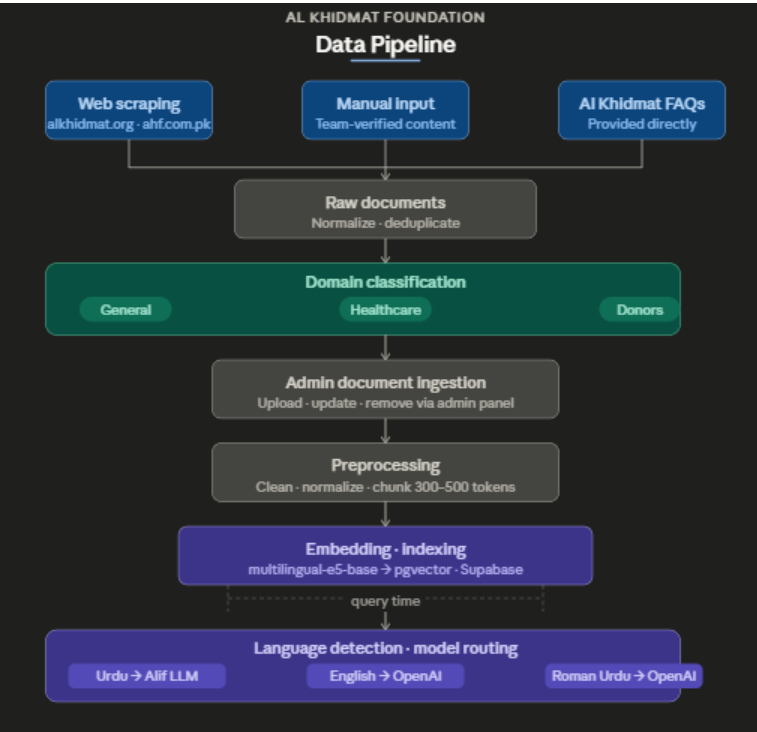
\includegraphics[width=0.8\textwidth]{chapters/data_pipeline.png}
    \caption{Data Pipeline Architecture}
    \label{fig:data-pipeline}
\end{figure}